%
% This is Chapter 1 file (chap1.tex)
%
\chapter{Introduction}

\section{SLEDS Background}

Infrared imaging and detection is used within countless modern services and industries. Infrared light exists outside the visible light spectrum and requires specialized equipment to project and detect signals. Infrared detection devices generally require high speed and precision that depend on reliable signals and input processing. These devices must therefore be thoroughly tested and calibrated. \par
A detector system must be "statically" and "dynamically" calibrated with an accurate infrared source \cite{marks}. A static calibration only requires basic equipment for testing radiance. Dynamic calibration is much more involved and requires a throrough understanding of the system in question. To dynamically test, the system is placed under more realistic and changing conditions such as having to react appropriately to moving objects or images. A common solution for testing in this capacity is the Infrared Scene Projector (IRSP) used to project infrared video signals that can be used to test infrared detection devices. \par
IRSPs display real time IR scenes that simulate a range of IR frequencies and patterns that a given device should operate under. Since infrared depends on physical information (temperature), generating IR input requires specialized hardware. This hardware is used to turn commands from the users into analog display signals as well as read feedback from the display device and adjust its own parameters accordingly. This "hardware-in-the-loop" approach can allow a system to accomodate physical effects or other issues within the display. Since infrared displays are analog devices, they cannot be precisely analyzed without some sort of readback and processing to view output. A typical system design is shown below. \par
\begin{figure}[!htb]
	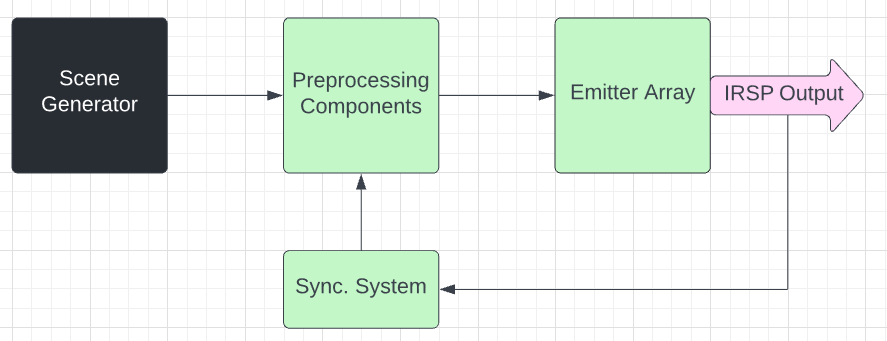
\includegraphics[width=0.7\textwidth]{irsp_block_diagram}
	\centering
	\caption{General IRSP architecture}
	\centering
\end{figure}
Testing is one of the most important aspects of any system design, as it is the bottleneck for how many reliable systems can be built \& validated. This work consists of a new approach to manually test the high-speed analog amplifier circuits within the system, as well as considerations \& redesigns for the next generation of these devices.

\section {Motivation}
IRSP performance is characterized by a multitude of factors. The major goals for any IRSP are to achieve high frame rates and resolution, although this generally involves multiple major developments across the system. The frame rate is directly tied to the rise time of individual pixels, which is fully dependent on the display architecture and physical properties. The temperature range represents different "colors" or ranges of IR light that the projector can display. Including more color bands increases the number of applications and devices to be tested with he IRSP. An ideal device has both high refresh rate, dynamic range, and resolution to provide an effective scene projection platform. \cite{marks} \par

Much of the IRSP market is dominated by resistor array devices. By heating up resistors (mapped to each pixel) to specific points with controlled current input, the device can simulate temperature output for an infrared image. This approach is effective but limited by the physical properties of all resistors. \cite{spie:2015} In modern IRSP scenarios, video must be refreshing quickly to provide the most realistic IR emissions.  High refresh rate in each pixel requires the driving component to be able to switch between any given values in a reliable amount of time. Resistors do not dissipate heat particularly quickly, limiting their rise time performance compared to other solutions. Many designs are forced to stay under 500 Hz. Increasing projected temperature deltas further stresses the switching capabilities of the driving component.\par

Since 2008, CVORG has been at the forefront of developing an Infrared LED-based IRSP with a full suite of custom hardware and software control. \cite{peyman} The success of the current iteration of the system has allowed further research and changes to the system that would expand on the technology's potential. Our technology is now targeting a 1024 x 1024 display at 2KHz in ideal conditions. \par

After being successfully developed into a minimum viable product, the IRSP platform was stable enough to reproduce and iterate on. The process of building and testing each component of the system promotes familiarity and understanding of the system architecutre as well as limitations the systems currently face. \par

A critical link in the system's loop is digital-to-analog conversion and amplification. These amplified analog signals are used to drive the display, making their integrity and low latency a top priority. \cite{tianne} As such, it was imperative to create reliable testing procedures for such components. The relevant systems, components \& design methodology for this portion of the system are described in detail below. \par
